\documentclass[11pt,a4paper]{article}

\usepackage[utf8]{inputenc}
\usepackage[T1]{fontenc}
\usepackage{mathptmx}
\usepackage[margin=2.4cm]{geometry}
\usepackage{amsmath,amssymb,amsthm}
\usepackage{graphicx}
\usepackage{caption}
\usepackage{subcaption}
\usepackage{booktabs}
\usepackage{xcolor}
\usepackage{microtype}
\usepackage{enumitem}
\usepackage[hidelinks]{hyperref}
\usepackage{titlesec}
\usepackage{fancyhdr}

\definecolor{accent}{RGB}{20,80,140}
\hypersetup{colorlinks=true,linkcolor=accent,citecolor=accent,urlcolor=accent}

\titleformat{\section}{\Large\bfseries\color{accent}}{\thesection}{0.7em}{}
\titleformat{\subsection}{\large\bfseries}{\thesubsection}{0.6em}{}

\pagestyle{fancy}
\fancyhf{}
\rhead{\small Delay-Aware Unicycle Rendezvous}
\lhead{\small Control of Multi-Robot Systems --- Project 2026}
\cfoot{\thepage}
\renewcommand{\headrulewidth}{0.4pt}

\newtheorem{proposition}{Proposition}
\newtheorem{remark}{Remark}

\newcommand{\R}{\mathbb{R}}
\newcommand{\Lap}{L}
\newcommand{\taucrit}{\tau_{\mathrm{crit}}}
\newcommand{\lammax}{\lambda_{\max}}

\title{\vspace{-1.2cm}\textbf{\color{accent}Delay-Aware Rendezvous of Unicycle\\ Multi-Robot Systems}\\[0.3cm]
\large Communication delays, nonholonomic constraints and the role of the critical delay $\taucrit$}
\author{Samuele Civale \and Matteo Zamponi \and Roberto~\textsc{[Surname]}}
\date{Control of Multi-Robot Systems --- Project 2026}

\begin{document}
\maketitle
\thispagestyle{fancy}

\begin{abstract}
\noindent
This report studies the \emph{rendezvous} problem for a team of nonholonomic unicycle robots
that exchange position information over a communication graph affected by a transport delay
$\tau$. The work combines two complementary viewpoints. First, we use the classical linear
full-state delayed-consensus model to derive the critical delay
\[
\taucrit = \frac{\pi}{2k\lambda_{\max}(L)},
\]
which is an exact stability threshold for the corresponding single-integrator consensus
system. Second, we use this value as a theoretical reference for the more realistic
nonholonomic unicycle system, where the desired consensus velocity cannot be applied directly
because each robot is constrained to move along its heading direction.

For this reason, $\taucrit$ should not be interpreted as a strict necessary and sufficient
stability boundary for the complete nonlinear unicycle dynamics. Rather, it provides a
meaningful baseline: it captures the delay margin of the underlying communication-consensus
layer and allows the simulations to be normalised through the ratio $\tau/\taucrit$. The
numerical experiments show that the unicycle rendezvous behaviour changes significantly
around this theoretical threshold, while the precise transition is affected by nonholonomic
constraints, heading dynamics, velocity saturation and the specific controller used to project
the consensus field onto admissible unicycle motions.

The study validates this interpretation through delay sweeps, topology and gain studies,
disconnected graphs, and several extensions such as leader--follower rendezvous, rigid
formations, obstacle avoidance, switching graphs, time-varying delays and edge-dependent
delays. The delay analysis is inspired by the consensus-with-communication-delays framework
of Seuret, Dimarogonas and Johansson~\cite{seuret2008consensus}, while the nonholonomic
rendezvous controller is motivated by the consensus-based rendezvous and formation laws for
unicycle robots proposed by Listmann, Masalawala and Adamy~\cite{listmann2009formation}.
\end{abstract}

\section{Introduction}

Rendezvous is one of the canonical problems in multi-robot coordination: a group of agents,
each measuring only relative information with respect to a set of neighbours, must agree on a
common meeting point using a distributed control law. When the agents are simple integrators
and information is exchanged instantaneously, the classical linear consensus protocol drives
the team to the centroid of the initial positions. Two features make the present study more
realistic and more challenging.

First, \textbf{communication is delayed}. Sensing, packetisation, transmission and processing
all introduce a latency $\tau$ between the instant a neighbour's position is generated and the
instant it is used in the control law. Delay is not a benign perturbation: beyond a precise
threshold it destabilises the very protocol that would otherwise guarantee convergence. A
central goal of this work is to derive that threshold, the \emph{critical delay} $\taucrit$,
and to explain its dependence on the controller gain and on the spectrum of the graph
Laplacian.

Second, the agents are \textbf{unicycles}, not integrators. The nonholonomic constraint
forbids instantaneous motion in an arbitrary direction: each robot can only move along its
current heading and steer. The consensus ``force'' produced by the delayed protocol must
therefore be reconciled with the admissible motion of the vehicle, which introduces a
nonlinearity absent from the linear reference model. This is why the nonholonomic part of the
project is treated as a controlled realisation of the consensus field, in line with
consensus-based rendezvous controllers for unicycle robots~\cite{listmann2009formation}.

The report is organised as follows. Section~\ref{sec:model} fixes the unicycle model and the
graph-theoretic notation. Section~\ref{sec:derivation} derives $\taucrit$ from a frequency
analysis of the delayed consensus protocol and discusses its meaning. Section~\ref{sec:roles}
compares the two delay models (full-state and neighbour-only). Section~\ref{sec:unicycle}
explains how the consensus field is realised on the unicycle. Section~\ref{sec:results}
presents the numerical validation, and Section~\ref{sec:extensions} the extensions.
Section~\ref{sec:conclusions} concludes.

\section{Model and preliminaries}
\label{sec:model}

\subsection{Unicycle kinematics}

We consider $N$ unicycle robots. The state of robot $i$ is the pose
$(x_i,y_i,\theta_i)$, with planar position $p_i=(x_i,y_i)\in\R^2$ and heading
$\theta_i$. The kinematics are
\begin{equation}
\dot{x}_i = v_i\cos\theta_i, \qquad
\dot{y}_i = v_i\sin\theta_i, \qquad
\dot{\theta}_i = \omega_i,
\label{eq:unicycle}
\end{equation}
where $v_i$ is the forward (linear) velocity and $\omega_i$ the angular velocity. The pair
$(v_i,\omega_i)$ is the control input, subject in the implementation to the saturation
$|v_i|\le v_{\max}$, $|\omega_i|\le\omega_{\max}$.

The nonholonomic constraint is made explicit by writing the velocity of the contact point as
$\dot p_i = v_i\,t_i$, with $t_i=(\cos\theta_i,\sin\theta_i)$ the unit tangent. The robot
cannot move along the normal direction $n_i=(-\sin\theta_i,\cos\theta_i)$ instantaneously;
lateral displacement is only achievable by first steering. This is the key structural
difference with respect to a single integrator $\dot p_i = u_i$, which can move in any
direction at will.

\subsection{Communication graph}

Information exchange is described by an undirected weighted graph
$\mathcal G=(\mathcal V,\mathcal E,A)$, with $\mathcal V=\{1,\dots,N\}$, edge set
$\mathcal E$ and symmetric adjacency matrix $A=[a_{ij}]$, $a_{ij}=a_{ji}\ge0$, $a_{ii}=0$.
Robot $j$ is a neighbour of $i$ (written $j\in\mathcal N_i$) iff $a_{ij}>0$. The degree matrix
is $D=\operatorname{diag}(d_1,\dots,d_N)$ with $d_i=\sum_j a_{ij}$, and the graph Laplacian is
\begin{equation}
\Lap = D - A.
\label{eq:laplacian}
\end{equation}
For an undirected graph $\Lap$ is symmetric positive semidefinite, so its eigenvalues are real
and can be ordered as
\[
0 = \lambda_1 \le \lambda_2 \le \cdots \le \lambda_N = \lammax(\Lap).
\]
The all-ones vector $\mathbf 1$ is always an eigenvector associated with $\lambda_1=0$, because
each row of $\Lap$ sums to zero. The second smallest eigenvalue $\lambda_2$ is the
\emph{algebraic connectivity}: $\lambda_2>0$ if and only if the graph is connected, and its
magnitude quantifies ``how connected'' the graph is, governing the asymptotic convergence
rate of consensus. The largest eigenvalue $\lammax$, as we will see, governs the delay
margin.

Throughout the baseline experiments we use a ring graph on $N=6$ nodes
(Figure~\ref{fig:ring}), for which $\lambda_2=1$, $\lammax=4$.

\begin{figure}[t]
\centering
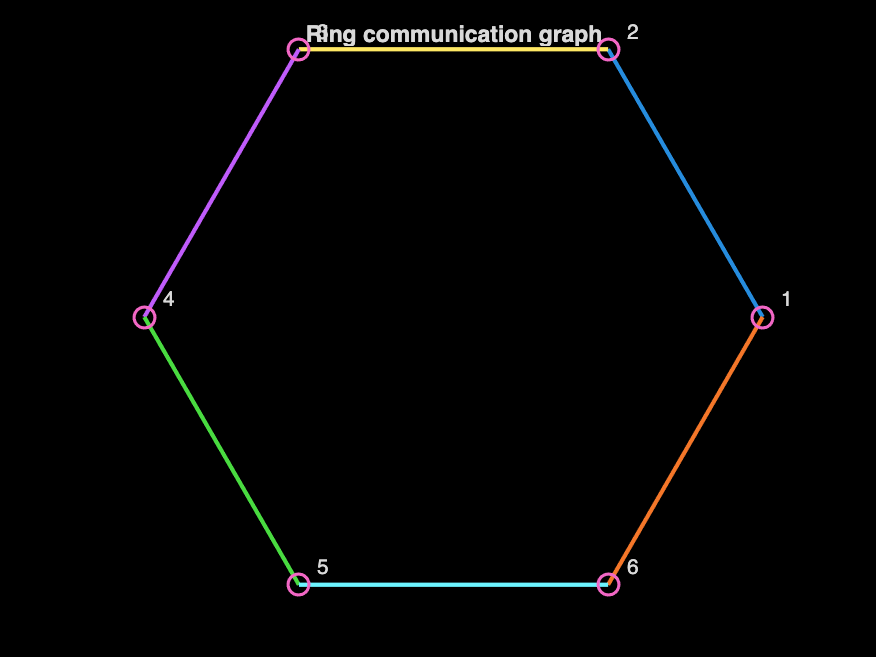
\includegraphics[width=0.52\textwidth]{figures/u00_ring_graph.png}
\caption{Baseline communication graph: a ring on $N=6$ nodes. For this graph
$\lambda_2(\Lap)=1$ and $\lammax(\Lap)=4$, which with the unit consensus gain $k=1$ yields a
reference critical delay $\taucrit=\pi/8\approx0.3927$~s.}
\label{fig:ring}
\end{figure}

\section{The delayed consensus protocol and the derivation of $\taucrit$}
\label{sec:derivation}

\subsection{Linear consensus without delay}

We begin with the linear reference model in which each agent is a single integrator,
$\dot p_i = u_i$, and the control is the standard consensus law
\begin{equation}
u_i = -k\sum_{j\in\mathcal N_i} a_{ij}\,(p_i - p_j),
\qquad k>0.
\label{eq:consensus_nodelay}
\end{equation}
Stacking the positions into $p=(p_1^\top,\dots,p_N^\top)^\top$ and using
\eqref{eq:laplacian}, the closed loop reads, componentwise in each Cartesian coordinate,
\begin{equation}
\dot p = -k\,\Lap\,p.
\label{eq:closed_nodelay}
\end{equation}
Because $\Lap\mathbf 1=0$, the average $\bar p=\frac1N\sum_i p_i$ is invariant
($\dot{\bar p}=-\tfrac kN\mathbf 1^\top\Lap p=0$), and on a connected graph all remaining modes
decay, so $p_i(t)\to\bar p(0)$ for all $i$: the agents rendezvous at the centroid. The decay
rates are exactly $k\lambda_2,\dots,k\lambda_N$, which is why $\lambda_2$ sets the slowest
mode.

\subsection{Introducing the transport delay}

Suppose now that the neighbour information used at time $t$ was generated at time $t-\tau$.
The \emph{full-state} delayed protocol replaces $p$ on the right-hand side of
\eqref{eq:closed_nodelay} by its delayed value:
\begin{equation}
\dot p(t) = -k\,\Lap\,p(t-\tau).
\label{eq:delayed_fullstate}
\end{equation}
This is a linear time-invariant delay-differential equation. Its stability is governed by the
spectrum of the associated characteristic equation, which we now diagonalise.

\subsection{Modal decomposition}

Since $\Lap$ is real symmetric, it admits an orthonormal eigenbasis: there is an orthogonal
matrix $V=[v_1,\dots,v_N]$ such that $V^\top \Lap V=\operatorname{diag}(\lambda_1,\dots,\lambda_N)$.
Projecting \eqref{eq:delayed_fullstate} onto this basis through the modal coordinates
$z=V^\top p$ decouples the system into $N$ scalar delay equations, one per eigenvalue:
\begin{equation}
\dot z_i(t) = -k\,\lambda_i\,z_i(t-\tau), \qquad i=1,\dots,N.
\label{eq:modal}
\end{equation}
The mode associated with $\lambda_1=0$ gives $\dot z_1=0$: it is the (conserved) average and
plays no role in stability. Every other mode is a scalar equation of the form
$\dot z = -a\,z(t-\tau)$ with $a=k\lambda_i>0$. The full system is stable if and only if
\emph{each} of these scalar modes is stable; the most demanding one will turn out to be the
mode with the largest $\lambda_i$, i.e.\ $\lammax$.

\subsection{Characteristic equation and the stability boundary}

Seek solutions of the scalar mode $\dot z = -a\,z(t-\tau)$ of the form $z(t)=e^{st}$. Substituting
gives the transcendental characteristic equation
\begin{equation}
s = -a\,e^{-s\tau}, \qquad a = k\lambda_i > 0.
\label{eq:char}
\end{equation}
For $\tau=0$ this reduces to $s=-a<0$: the mode is stable, consistent with the delay-free
analysis. As $\tau$ grows the roots $s(\tau)$ move continuously in the complex plane. The
system loses stability precisely when a root first reaches the imaginary axis, i.e.\ when a
purely imaginary root $s=j\omega$ appears. Substituting $s=j\omega$ into \eqref{eq:char},
\begin{equation}
j\omega = -a\,e^{-j\omega\tau}
        = -a\bigl(\cos\omega\tau - j\sin\omega\tau\bigr).
\label{eq:char_imag}
\end{equation}
Separating real and imaginary parts yields the two conditions
\begin{align}
\text{(real)}      &\quad 0 = -a\cos\omega\tau, \label{eq:real}\\
\text{(imaginary)} &\quad \omega = a\sin\omega\tau. \label{eq:imag}
\end{align}
Since $a>0$, equation \eqref{eq:real} forces $\cos\omega\tau=0$, hence
$\omega\tau = \pi/2 \;(+\,m\pi)$. The first crossing---the one that determines the stability
margin---corresponds to $\omega\tau=\pi/2$. Taking $\omega>0$, equation \eqref{eq:imag} then
gives $\omega = a\sin(\pi/2) = a$. Combining the two,
\begin{equation}
\omega = a, \qquad \omega\tau = \frac{\pi}{2}
\;\;\Longrightarrow\;\;
\tau = \frac{\pi}{2a} = \frac{\pi}{2\,k\lambda_i}.
\label{eq:tau_mode}
\end{equation}
Thus the mode with eigenvalue $\lambda_i$ becomes marginally stable at delay
$\pi/(2k\lambda_i)$, and is unstable for larger delays. The whole system is stable only as long
as \emph{all} modes are stable, i.e.\ up to the \emph{smallest} of these per-mode thresholds,
which is attained by the \emph{largest} eigenvalue. Therefore the critical delay of the
networked system is
\begin{equation}
\boxed{\;\taucrit = \dfrac{\pi}{2\,k\,\lammax(\Lap)}\;}
\label{eq:taucrit}
\end{equation}

\begin{proposition}[Critical delay]
Consider the delayed consensus system \eqref{eq:delayed_fullstate} on a connected undirected
graph with gain $k>0$. All non-average modes are asymptotically stable if $0\le\tau<\taucrit$,
with $\taucrit$ given by \eqref{eq:taucrit}, and at least one mode is marginally stable at
$\tau=\taucrit$; for $\tau>\taucrit$ the mode associated with $\lammax$ is unstable.
\end{proposition}

\begin{remark}[Role of $\taucrit$ in the nonholonomic system]
The critical delay $\taucrit$ in \eqref{eq:taucrit} is derived for the linear delayed consensus
dynamics of single-integrator agents. Therefore, it is an exact stability threshold for the
underlying full-state delayed consensus layer, not for the complete nonlinear unicycle model.
In the unicycle case, the desired consensus velocity must be converted into admissible inputs
$(v_i,\omega_i)$, and this introduces heading dynamics, projection effects, saturations and
other nonlinearities.

Consequently, in this report $\taucrit$ is used as a theoretical baseline rather than as a
strict necessary and sufficient stability condition for the nonholonomic closed-loop system.
Its value remains important because the unicycle controller is built around the same consensus
vector field: when $\tau/\taucrit$ approaches or exceeds one, the delayed communication layer
tends to generate oscillatory or divergent behaviours, which are then reflected in the
nonholonomic trajectories. The simulations should therefore be read as a numerical validation
of how the theoretical delay margin of the consensus layer manifests itself in the more
realistic unicycle rendezvous problem.
\end{remark}

\begin{remark}[Physical reading of the threshold]
The product $k\lammax$ has the units of a rate (inverse time); it is the fastest closed-loop
rate the network tries to impose. Its reciprocal $1/(k\lammax)$ is the corresponding time
constant, and the delay margin \eqref{eq:taucrit} is a quarter period
($\pi/2$ in phase) of the oscillation that this fastest mode would sustain at the boundary.
Intuitively, a delay equal to a quarter of the natural oscillation period turns the corrective
action into a destabilising, out-of-phase action: the agent keeps reacting to where its
neighbours \emph{were}, overshooting and feeding an oscillation that grows without bound.
\end{remark}

\subsection{Design consequences}

Equation \eqref{eq:taucrit} exposes the two levers that set the delay margin.

\paragraph{Gain.} The margin is inversely proportional to $k$: a more aggressive controller
converges faster when there is no delay but tolerates \emph{less} delay. Halving $k$ doubles
$\taucrit$. This trade-off between nominal speed and delay robustness is verified numerically
in Section~\ref{sec:gain}.

\paragraph{Topology.} The margin is inversely proportional to $\lammax(\Lap)$. Denser graphs
and larger edge weights raise $\lammax$ and hence \emph{shrink} the delay margin. A complete
graph $K_N$ with unit weights has $\lammax=N$, so its margin decreases as the team grows,
whereas a sparse path graph has the smallest $\lammax$ among connected topologies on the same
nodes and therefore the largest margin. Connectivity ($\lambda_2$) speeds up convergence but
it is $\lammax$, not $\lambda_2$, that limits the delay.

\section{The two delay models and the role of $\taucrit$}
\label{sec:roles}

The derivation above used the \emph{full-state} model \eqref{eq:delayed_fullstate}, in which
\emph{both} the agent's own state and its neighbours' states enter delayed. A second, often
more realistic, model delays \emph{only the information that physically travels over the
network}---the neighbours' states---while each agent uses its \emph{own} current position
without delay (it is locally available). This \emph{neighbour-only} protocol is
\begin{equation}
u_i(t) = -k\sum_{j\in\mathcal N_i} a_{ij}\bigl(p_i(t) - p_j(t-\tau)\bigr),
\label{eq:neighbor_only}
\end{equation}
or, in stacked form, $\dot p(t) = -k\bigl(D\,p(t) - A\,p(t-\tau)\bigr)$. The undelayed term
$-kD\,p(t)$ adds instantaneous damping that the full-state model lacks, which substantially
enlarges the delay margin. The full-state threshold \eqref{eq:taucrit} therefore acts as a
\emph{conservative reference}: it is exact for \eqref{eq:delayed_fullstate}, and for
\eqref{eq:neighbor_only} the true margin is larger, so $\taucrit$ remains a meaningful and safe
yardstick against which to normalise all delays in the experiments.

The role of $\taucrit$ can thus be summarised as follows. It is the \emph{phase margin of the
linear consensus network expressed as a time}: a single number, computable from the gain and
the graph spectrum alone, that predicts when delayed cooperation flips from stabilising to
destabilising in the reference model. In the nonholonomic unicycle system it is not used as an
exact boundary, but as the theoretical scale with which all delays are compared. All
experiments below therefore report the dimensionless ratio $\tau/\taucrit$, which makes
results comparable across graphs of very different size and density and clarifies how the
linear delay margin appears in the nonlinear unicycle simulations.

\section{From the consensus field to the unicycle}
\label{sec:unicycle}

The protocols \eqref{eq:delayed_fullstate} and \eqref{eq:neighbor_only} produce, at each
instant, a desired Cartesian velocity $u_i\in\R^2$ for agent $i$. A single integrator could
apply it directly; a unicycle cannot, because of the nonholonomic constraint. Two controllers
are used to reconcile $u_i$ with \eqref{eq:unicycle}.

\paragraph{Vector-field tracking controller.} The desired velocity is treated as a reference
to be tracked in direction and magnitude. With heading error
$e_\theta=\operatorname{atan2}(u_{i,y},u_{i,x})-\theta_i$ wrapped to $(-\pi,\pi]$, the inputs are
\begin{equation}
v_i = k_v\,\|u_i\|\,\max\{0,\cos e_\theta\}, \qquad
\omega_i = k_\theta\,e_\theta .
\label{eq:vf}
\end{equation}
The robot drives forward only when it roughly faces the target direction (the
$\max\{0,\cos e_\theta\}$ gate) and steers proportionally to the heading error.

\paragraph{Force-projection (``paper'') controller.} Inspired by potential-field rendezvous
laws for nonholonomic agents, the vector $u_i$ is interpreted as an interaction force and is
\emph{projected} onto the admissible direction of motion $t_i$:
\begin{equation}
v_i = k_v\, u_i^\top t_i, \qquad
\omega_i = k_\theta\,e_\theta .
\label{eq:paper}
\end{equation}
Only the component of the force along the current heading produces translation; the orthogonal
component is rejected and handled by steering. This is the default controller and the one most
faithful to the reference papers.

In both cases the heading dynamics and the saturation are genuine nonlinearities, so the
linear threshold \eqref{eq:taucrit} is no longer exact for the unicycle. This is the main
reason why $\taucrit$ is interpreted as a theoretical reference for the nonholonomic system,
rather than as a formal stability theorem for the complete closed loop. It remains, however,
an excellent organising quantity: as the experiments show, behaviour changes \emph{character}
in the neighbourhood of $\tau/\taucrit\approx1$, even though the precise crossing is shifted by
the nonlinearity.

\section{Numerical validation}
\label{sec:results}

All experiments use the parameters $k=1$, $k_v=1$, $k_\theta=3$, $v_{\max}=1.5$,
$\omega_{\max}=4$, integration step $dt=0.02$~s, on the ring graph of Figure~\ref{fig:ring}
unless stated otherwise. Convergence is measured by the root-mean-square (RMS) disagreement
\begin{equation}
\delta(t) = \sqrt{\tfrac1N\textstyle\sum_{i}\|p_i(t)-\bar p(t)\|^2},
\label{eq:disagreement}
\end{equation}
the spatial spread of the team about its centroid; rendezvous corresponds to
$\delta(t)\to0$.

\subsection{Baseline rendezvous}

With a sub-critical delay $\tau=0.3\,\taucrit$, the full-state unicycle team rendezvouses
cleanly (Figure~\ref{fig:u01}). The recorded final disagreement is
$\delta_\infty\approx8.3\times10^{-9}$, with a convergence time of $6.22$~s and a final
centroid at $(0.284,0.108)$---close to the centroid of the initial positions, as the theory
predicts for small delay.

\begin{figure}[t]
\centering
\begin{subfigure}{0.48\textwidth}
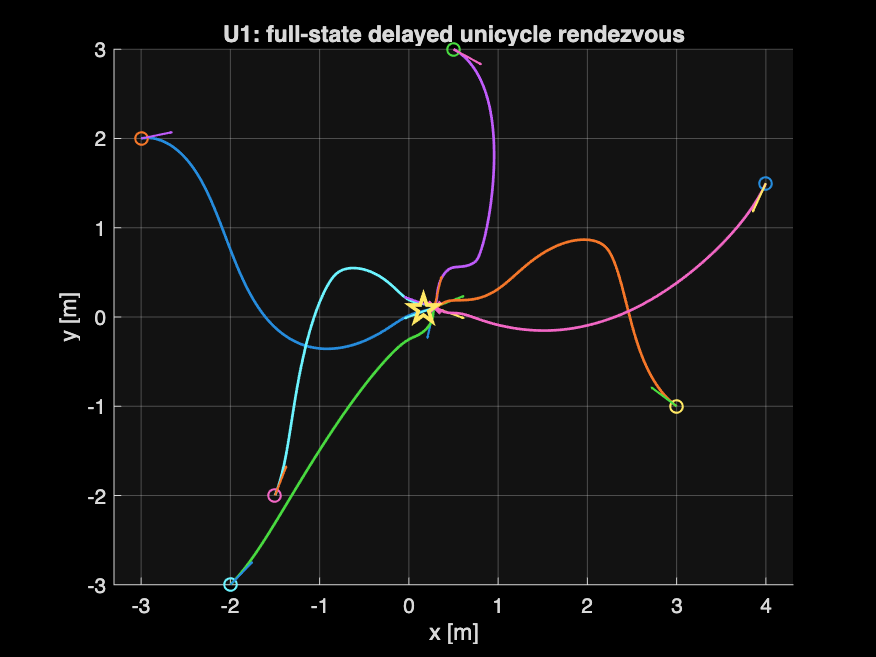
\includegraphics[width=\textwidth]{figures/u01_full_state_trajectories.png}
\caption{Trajectories.}
\end{subfigure}\hfill
\begin{subfigure}{0.48\textwidth}
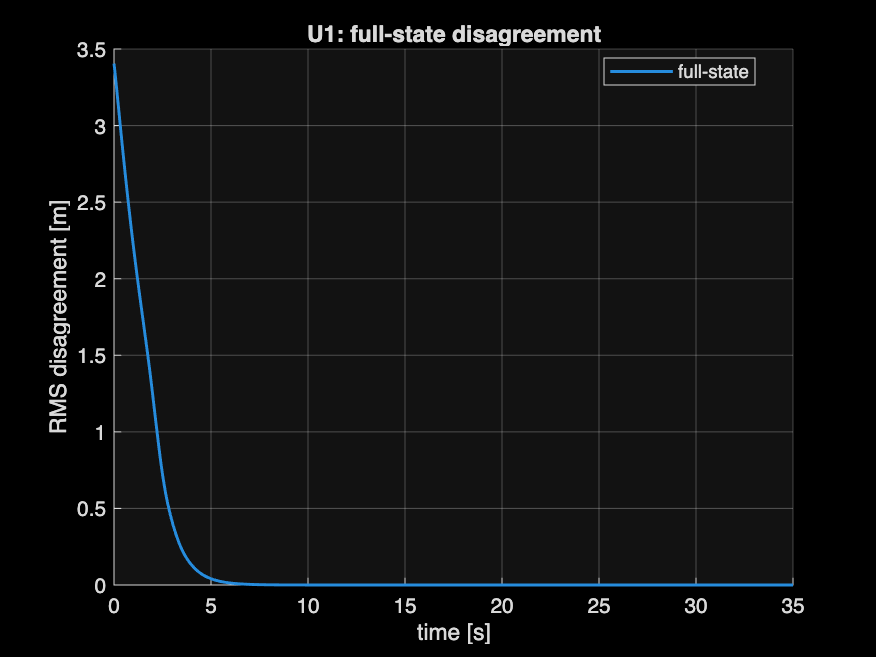
\includegraphics[width=\textwidth]{figures/u01_full_state_disagreement.png}
\caption{RMS disagreement $\delta(t)$.}
\end{subfigure}
\caption{Baseline full-state rendezvous at $\tau=0.3\,\taucrit$. The six robots
(arrows show initial and final headings) converge to a common point; the disagreement decays
monotonically to numerical zero.}
\label{fig:u01}
\end{figure}

\subsection{Delay sweep: the threshold in action}
\label{sec:sweep}

The single most important experiment sweeps $\tau$ from $0$ to $2\,\taucrit$ for both delay
models. Table~\ref{tab:sweep} reports the final disagreement and convergence time, and
Figure~\ref{fig:u03} visualises the contrast.

\begin{table}[h]
\centering
\caption{Delay sweep on the ring graph. Final RMS disagreement and convergence time as a
function of $\tau/\taucrit$, for the two delay models. ``---'' denotes no convergence within
the horizon.}
\label{tab:sweep}
\small
\begin{tabular}{lcccc}
\toprule
& \multicolumn{2}{c}{\textbf{full-state}} & \multicolumn{2}{c}{\textbf{neighbour-only}}\\
\cmidrule(lr){2-3}\cmidrule(lr){4-5}
$\tau/\taucrit$ & $\delta_\infty$ & $t_c$ [s] & $\delta_\infty$ & $t_c$ [s]\\
\midrule
0.00 & $9.5\times10^{-9}$ & 6.76 & $9.5\times10^{-9}$ & 6.76\\
0.25 & $8.7\times10^{-9}$ & 6.32 & $9.5\times10^{-9}$ & 7.30\\
0.50 & $6.5\times10^{-9}$ & 5.88 & $9.6\times10^{-9}$ & 7.90\\
0.75 & $0.609$ & --- & $9.6\times10^{-9}$ & 8.52\\
0.95 & $0.684$ & --- & $9.7\times10^{-9}$ & 9.02\\
1.05 & $0.722$ & --- & $9.8\times10^{-9}$ & 9.28\\
1.20 & $0.778$ & --- & $9.8\times10^{-9}$ & 9.64\\
1.50 & $0.890$ & --- & $1.4\times10^{-4}$ & 10.48\\
2.00 & $1.078$ & --- & $0.073$ & ---\\
\bottomrule
\end{tabular}
\end{table}

Three observations stand out. First, the \textbf{full-state model collapses across the
predicted region}: it converges for $\tau\le0.5\,\taucrit$ and fails to rendezvous from
$0.75\,\taucrit$ onward, with the residual disagreement growing monotonically with $\tau$.
That the practical crossing occurs somewhat below the ideal $\tau=\taucrit$ is exactly the
expected effect of the unicycle nonlinearity and the finite integration step: the linear
$\taucrit$ is an upper bound on the achievable margin, approached but not reached by the
nonholonomic system. Second, the \textbf{neighbour-only model is dramatically more robust}: it
still rendezvouses essentially perfectly at $\tau=1.2\,\taucrit$ and only begins to degrade
near $2\,\taucrit$, confirming the extra damping argument of Section~\ref{sec:roles}. Third,
within the convergent regime, \textbf{larger delay slows convergence} (the neighbour-only
$t_c$ grows from $6.8$ to $10.5$~s): even when stability is preserved, latency has a cost.

\begin{figure}[t]
\centering
\begin{subfigure}{0.48\textwidth}
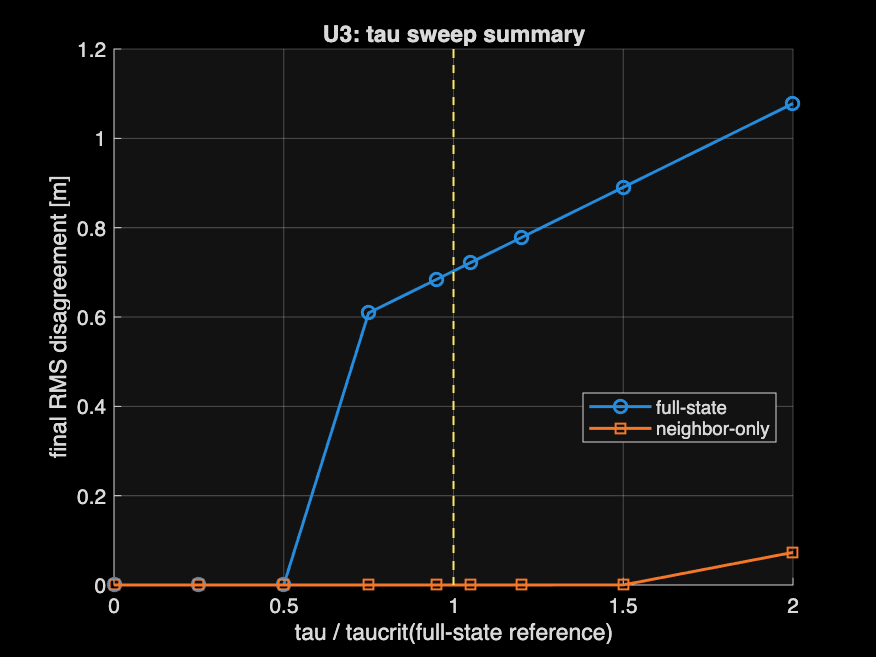
\includegraphics[width=\textwidth]{figures/u03_tau_sweep_summary.png}
\caption{Final disagreement vs $\tau/\taucrit$ (log scale).}
\end{subfigure}\hfill
\begin{subfigure}{0.48\textwidth}
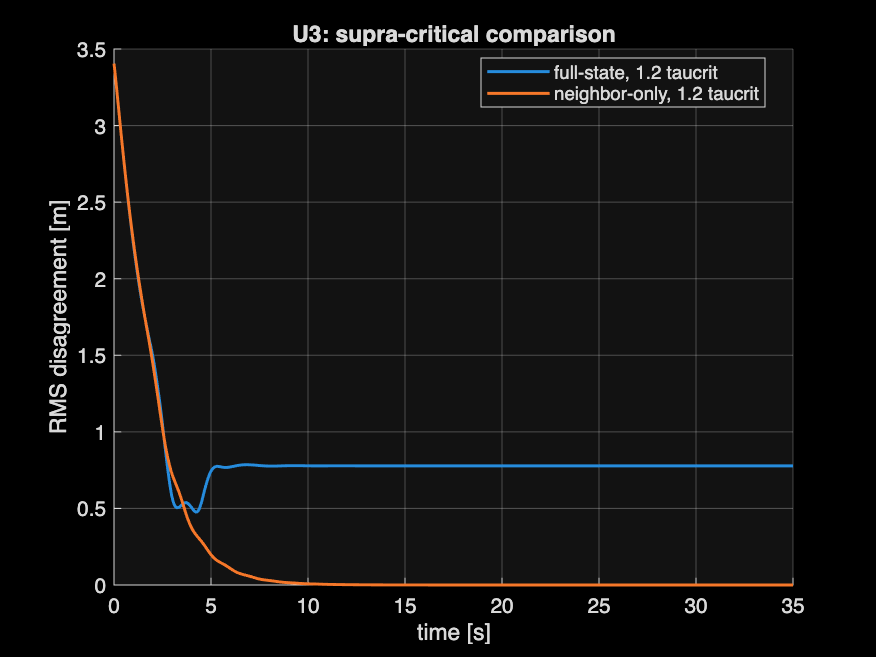
\includegraphics[width=\textwidth]{figures/u03_supracritical_curves.png}
\caption{Disagreement curves at $\tau=1.2\,\taucrit$.}
\end{subfigure}
\caption{Delay sweep, full-state vs neighbour-only. (a) The full-state curve jumps by orders
of magnitude as $\tau$ crosses the threshold (dashed line at $\tau/\taucrit=1$), while the
neighbour-only curve stays near zero far beyond it. (b) At $1.2\,\taucrit$ the full-state mode
saturates at a large residual while the neighbour-only team still converges.}
\label{fig:u03}
\end{figure}

\subsection{Topology}

Equation \eqref{eq:taucrit} predicts that the delay margin is set by $\lammax$, hence by the
density of the graph. Figure~\ref{fig:u04} compares path, ring, star and complete topologies
at a common relative delay $\tau=0.5\,\taucrit$ (each graph normalised by its \emph{own}
$\taucrit$). The denser graphs (star, complete) have the largest $\lammax$ and therefore the
smallest absolute margin; the sparse path has the smallest $\lammax$ and the largest margin.
At equal $\tau/\taucrit$ all connected topologies rendezvous, but their convergence times order
themselves according to algebraic connectivity $\lambda_2$, the denser graphs being faster.

\begin{figure}[t]
\centering
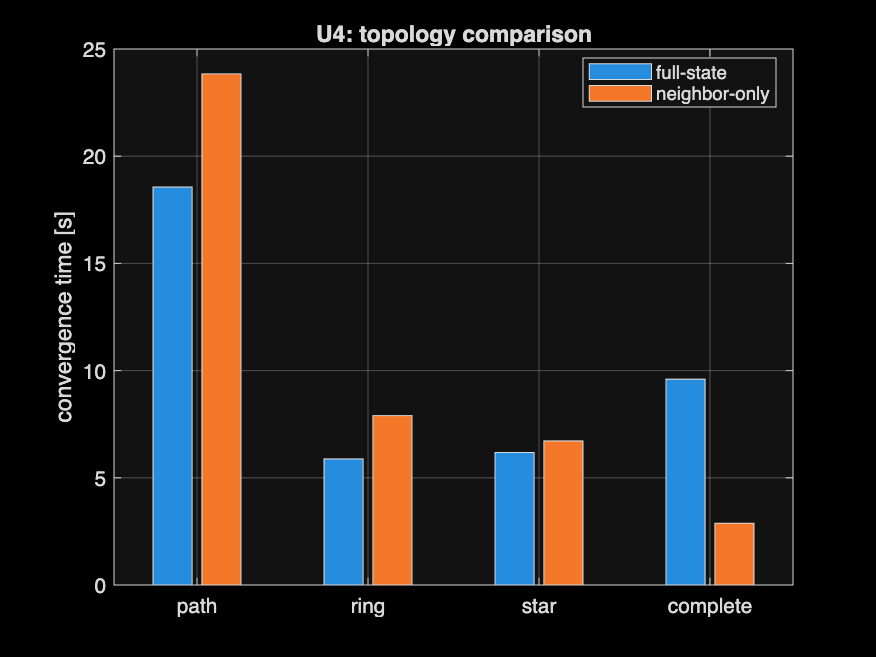
\includegraphics[width=0.62\textwidth]{figures/u04_topology_summary.png}
\caption{Topology comparison at $\tau=0.5\,\taucrit$ (each graph uses its own $\taucrit$).
Convergence time per topology for the two delay models; denser graphs converge faster but, in
absolute terms, tolerate a smaller delay because of their larger $\lammax$.}
\label{fig:u04}
\end{figure}

\subsection{Gain versus delay margin}
\label{sec:gain}

To isolate the role of $k$ we vary the consensus gain and, for each value, run at a delay
fixed at $0.8\,\taucrit(k)$, i.e.\ at a constant \emph{relative} delay. Since
$\taucrit\propto1/k$, increasing $k$ shrinks the absolute admissible delay in exact inverse
proportion (Figure~\ref{fig:u11}). This is the practical statement of the speed/robustness
trade-off: one cannot make the network arbitrarily fast and arbitrarily delay-tolerant at the
same time.

\begin{figure}[t]
\centering
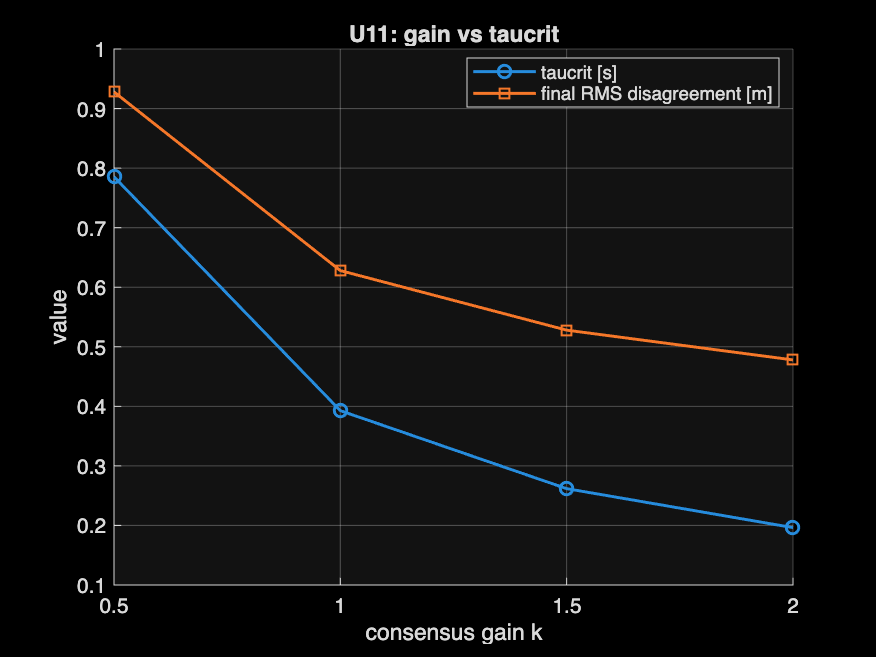
\includegraphics[width=0.62\textwidth]{figures/u11_gain_vs_taucrit.png}
\caption{Effect of the consensus gain $k$. The critical delay $\taucrit$ (left axis) falls as
$1/k$, confirming \eqref{eq:taucrit}; the final disagreement stays small because each run is
kept at the same relative delay $0.8\,\taucrit(k)$.}
\label{fig:u11}
\end{figure}

\subsection{Disconnected graph}

When the graph is not connected, $\lambda_2=0$ and global rendezvous is impossible: the
average is conserved \emph{within each component} but not across components. Figure~\ref{fig:u08}
shows a graph made of three disjoint pairs; each pair rendezvouses to its own local meeting
point, producing three clusters rather than one. This is the spatial signature of
$\lambda_2=0$ and a useful negative control: it confirms that connectivity, not merely the
control law, is what enables global agreement.

\begin{figure}[t]
\centering
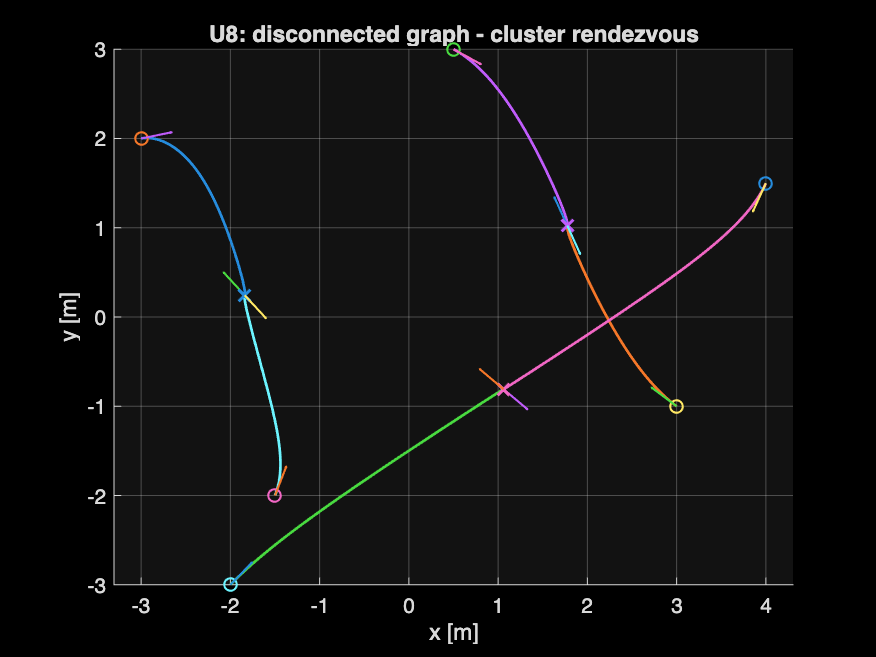
\includegraphics[width=0.55\textwidth]{figures/u08_disconnected_full_state.png}
\caption{Disconnected graph (three disjoint pairs). Each connected component reaches its own
local rendezvous point; no global agreement is possible because $\lambda_2=0$.}
\label{fig:u08}
\end{figure}

\section{Extensions}
\label{sec:extensions}

The same delayed-consensus core is reused, with additional terms, to cover a range of more
realistic coordination tasks. We highlight four representative ones.

\subsection{Leader--follower with a moving target}

One robot is designated leader and is driven to track a moving reference
$r(t)=1.8\,(\cos0.18t,\sin0.18t)$, while the others follow through the delayed neighbour-only
consensus. The team forms a cohesive group that trails the leader along its circular path
(Figure~\ref{fig:u15}); the follower spread settles to a small steady value, showing that
delayed consensus is compatible with a non-stationary objective.

\begin{figure}[t]
\centering
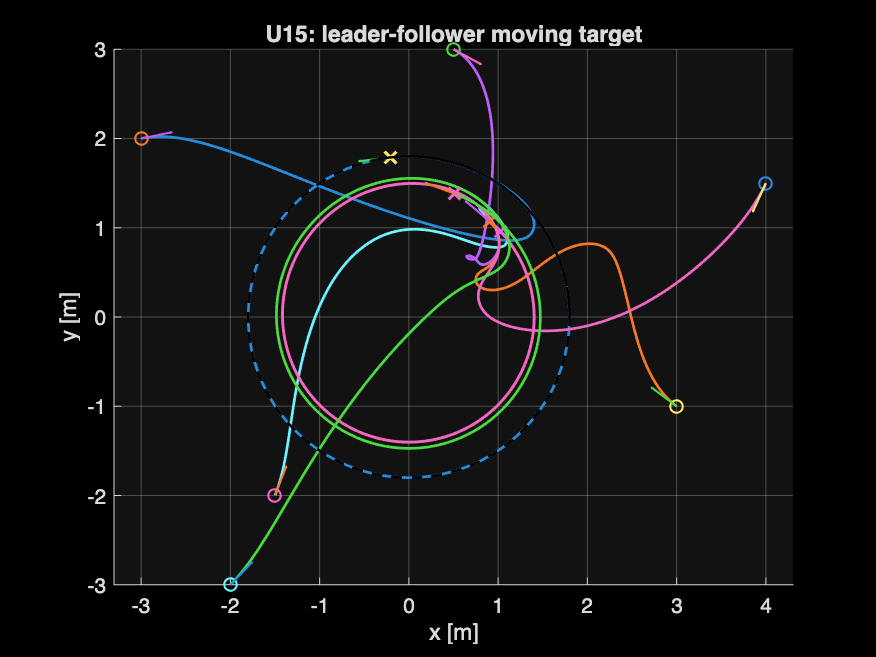
\includegraphics[width=0.55\textwidth]{figures/u15_leader_follower_trajectories.png}
\caption{Leader--follower with a moving target. The leader (driven by an external reference)
sweeps a circle; the followers track it cohesively through delayed consensus.}
\label{fig:u15}
\end{figure}

\subsection{Rigid formation}

Applying consensus to \emph{shifted} coordinates $q_i=p_i-\rho_i$, where $\rho_i$ are
prescribed offsets, turns rendezvous into a formation: the team agrees on the $q_i$, hence the
$p_i$ settle on the desired geometric pattern about an anchor point
(Figure~\ref{fig:u16}). The delay analysis carries over unchanged, since the offset is a
constant exogenous term.

\begin{figure}[t]
\centering
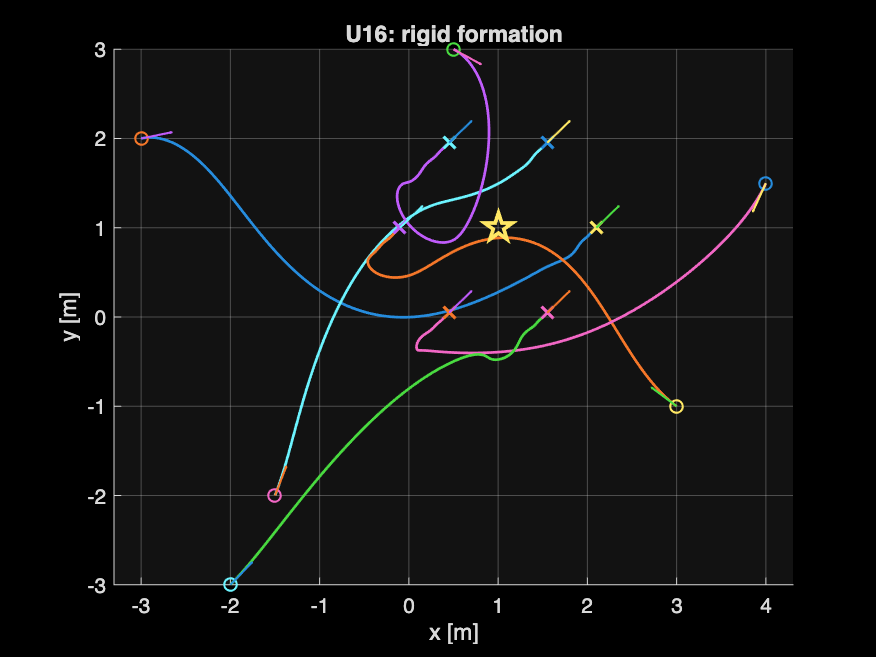
\includegraphics[width=0.55\textwidth]{figures/u16_formation_trajectories.png}
\caption{Rigid formation. Consensus on offset coordinates drives the robots onto a polygonal
formation centred at the anchor point (star marker).}
\label{fig:u16}
\end{figure}

\subsection{Obstacle and inter-robot collision avoidance}

Continuous repulsive terms are added for a circular obstacle and for pairwise robot
proximity. The team rendezvouses while bending its paths around the obstacle and maintaining a
positive minimum inter-robot clearance (Figure~\ref{fig:u19}). The avoidance terms are local
and vanish away from the danger zones, so they do not affect the delayed-consensus behaviour
in free space.

\begin{figure}[t]
\centering
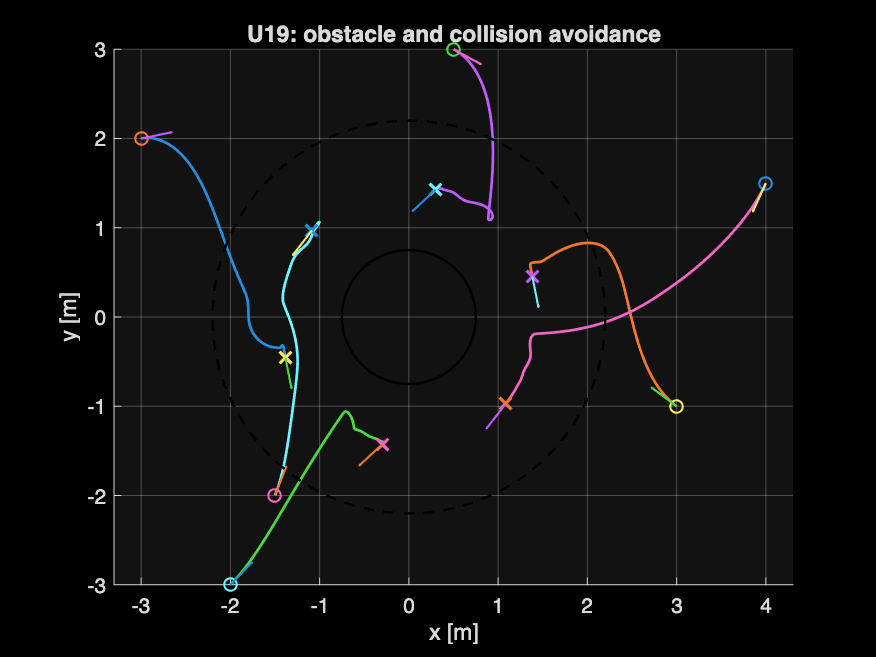
\includegraphics[width=0.55\textwidth]{figures/u19_avoidance_trajectories.png}
\caption{Obstacle and collision avoidance. Solid and dashed circles mark the obstacle and its
influence region; trajectories deflect smoothly around it while the team still rendezvouses.}
\label{fig:u19}
\end{figure}

\subsection{Switching graph and time-varying delay}

Two further stress tests probe the theory's assumptions. In the first, the graph is rebuilt at
every step from the robots' positions (a proximity graph), so the topology---and hence
$\lambda_2(L(t))$ and $\lammax(L(t))$---changes during the motion (Figure~\ref{fig:u20}). The
team still converges as long as the graph remains connected often enough, and the recorded
$\lambda_2(t)$ stays positive. In the second, the delay itself is made time-varying,
$\tau(t)=\taucrit\,\beta\,(1+\alpha\sin2\pi f t)$, including a profile whose peak crosses
$\taucrit$ (Figure~\ref{fig:u22}). The neighbour-only model tolerates excursions above the
nominal threshold, consistent with its larger true margin, whereas the full-state model is
sensitive to them.

\begin{figure}[t]
\centering
\begin{subfigure}{0.48\textwidth}
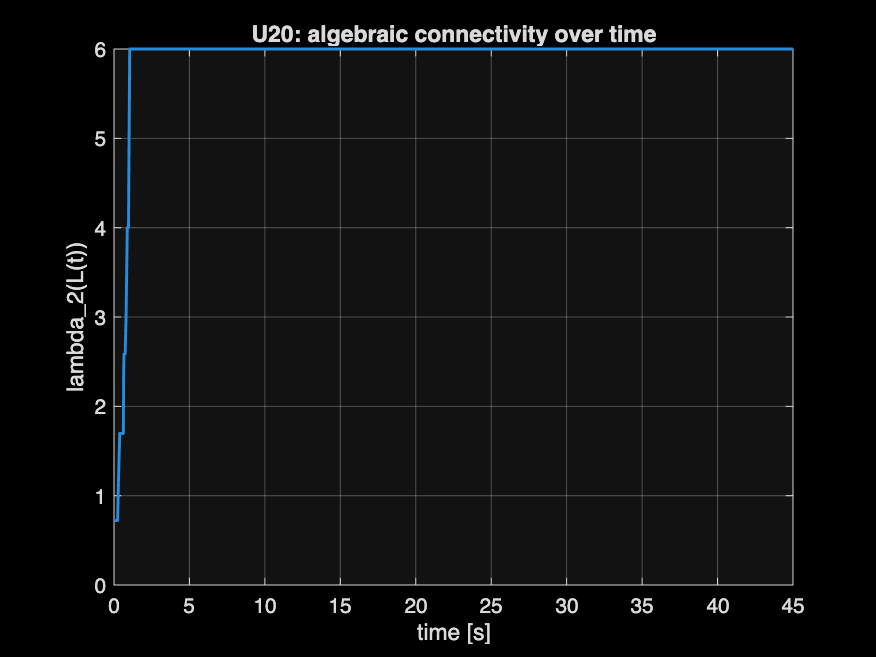
\includegraphics[width=\textwidth]{figures/u20_switching_graph_lambda2.png}
\caption{Algebraic connectivity $\lambda_2(L(t))$ of the switching proximity graph.}
\end{subfigure}\hfill
\begin{subfigure}{0.48\textwidth}
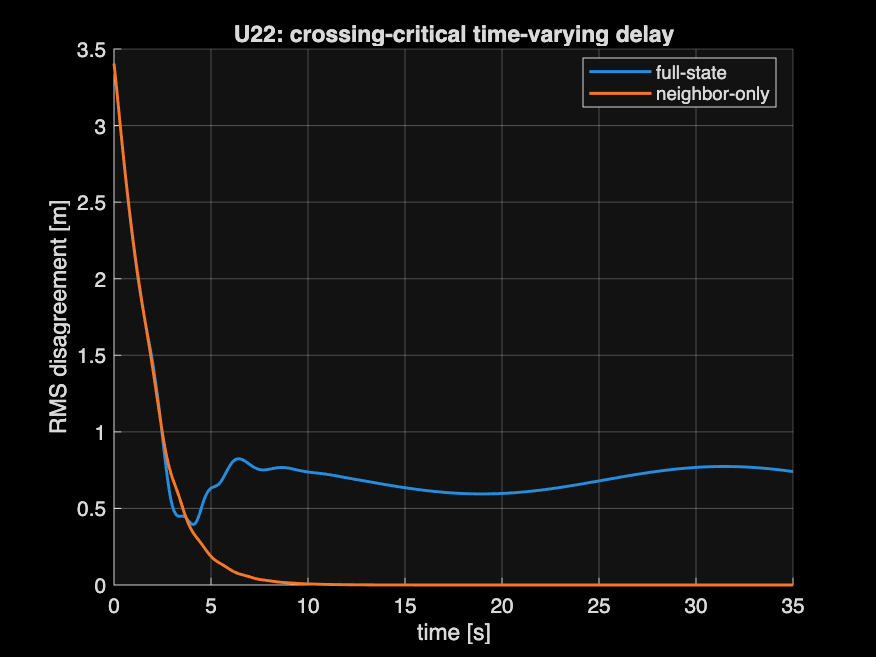
\includegraphics[width=\textwidth]{figures/u22_crossing_critical_curves.png}
\caption{Disagreement under a delay that crosses $\taucrit$.}
\end{subfigure}
\caption{Robustness to a time-varying network. (a) As the proximity graph switches, its
algebraic connectivity varies but stays positive, preserving convergence. (b) Under a
sinusoidal delay peaking above $\taucrit$, the neighbour-only protocol remains well behaved.}
\label{fig:u20}\label{fig:u22}
\end{figure}

\section{Conclusions}
\label{sec:conclusions}

We derived, from a frequency-domain analysis of the linear full-state delayed consensus
protocol, the critical communication delay $\taucrit=\pi/(2k\lammax(\Lap))$, and we explained
its role as the time expression of the network's phase margin. This quantity is exact for the
single-integrator consensus layer, where it separates convergent from divergent cooperation,
and it makes transparent the two design levers---gain and topology density---showing that
aggressiveness and delay robustness are inversely related.

Transferring the consensus field to nonholonomic unicycles through a force-projection
controller, we used $\taucrit$ as a theoretical baseline rather than as an exact stability
condition for the complete nonlinear system. The delay sweep confirms that this baseline is
still informative: the full-state unicycle protocol loses rendezvous as $\tau$ approaches the
linear threshold (slightly earlier, as expected from the unicycle nonlinearity), while the
neighbour-only protocol---thanks to its instantaneous self-damping---remains robust well
beyond it. Topology, gain, and disconnected-graph experiments confirm the dependence on
$\lammax$ and $\lambda_2$, and a suite of extensions (leader--follower, rigid formations,
obstacle avoidance, switching graphs and time-varying delays) shows that the delayed-consensus
core extends gracefully to realistic coordination tasks. The overarching practical message is
to normalise every delay by $\taucrit$, to interpret it as the delay margin of the underlying
consensus layer, and, whenever the architecture permits, to prefer the neighbour-only protocol
for its substantially larger delay margin.


\begin{thebibliography}{9}

\bibitem{seuret2008consensus}
A. Seuret, D. V. Dimarogonas, and K. H. Johansson,
``Consensus under Communication Delays,''
in \emph{Proceedings of the 47th IEEE Conference on Decision and Control},
Cancun, Mexico, 2008, pp. 4922--4927.

\bibitem{listmann2009formation}
K. D. Listmann, M. V. Masalawala, and J. Adamy,
``Consensus for Formation Control of Nonholonomic Mobile Robots,''
in \emph{Proceedings of the IEEE International Conference on Robotics and Automation},
Kobe, Japan, 2009, pp. 3886--3891.

\end{thebibliography}

\end{document}